\section{Experimental Setup}

This section describes the experimental setup, providing details about data splits, preprocessing steps, hyperparameter tuning, computational resources, and the tools and libraries utilized. The goal is to ensure reproducibility, transparency, and alignment with established best practices in machine learning research.
\begin{figure*}[t]
    \centering
    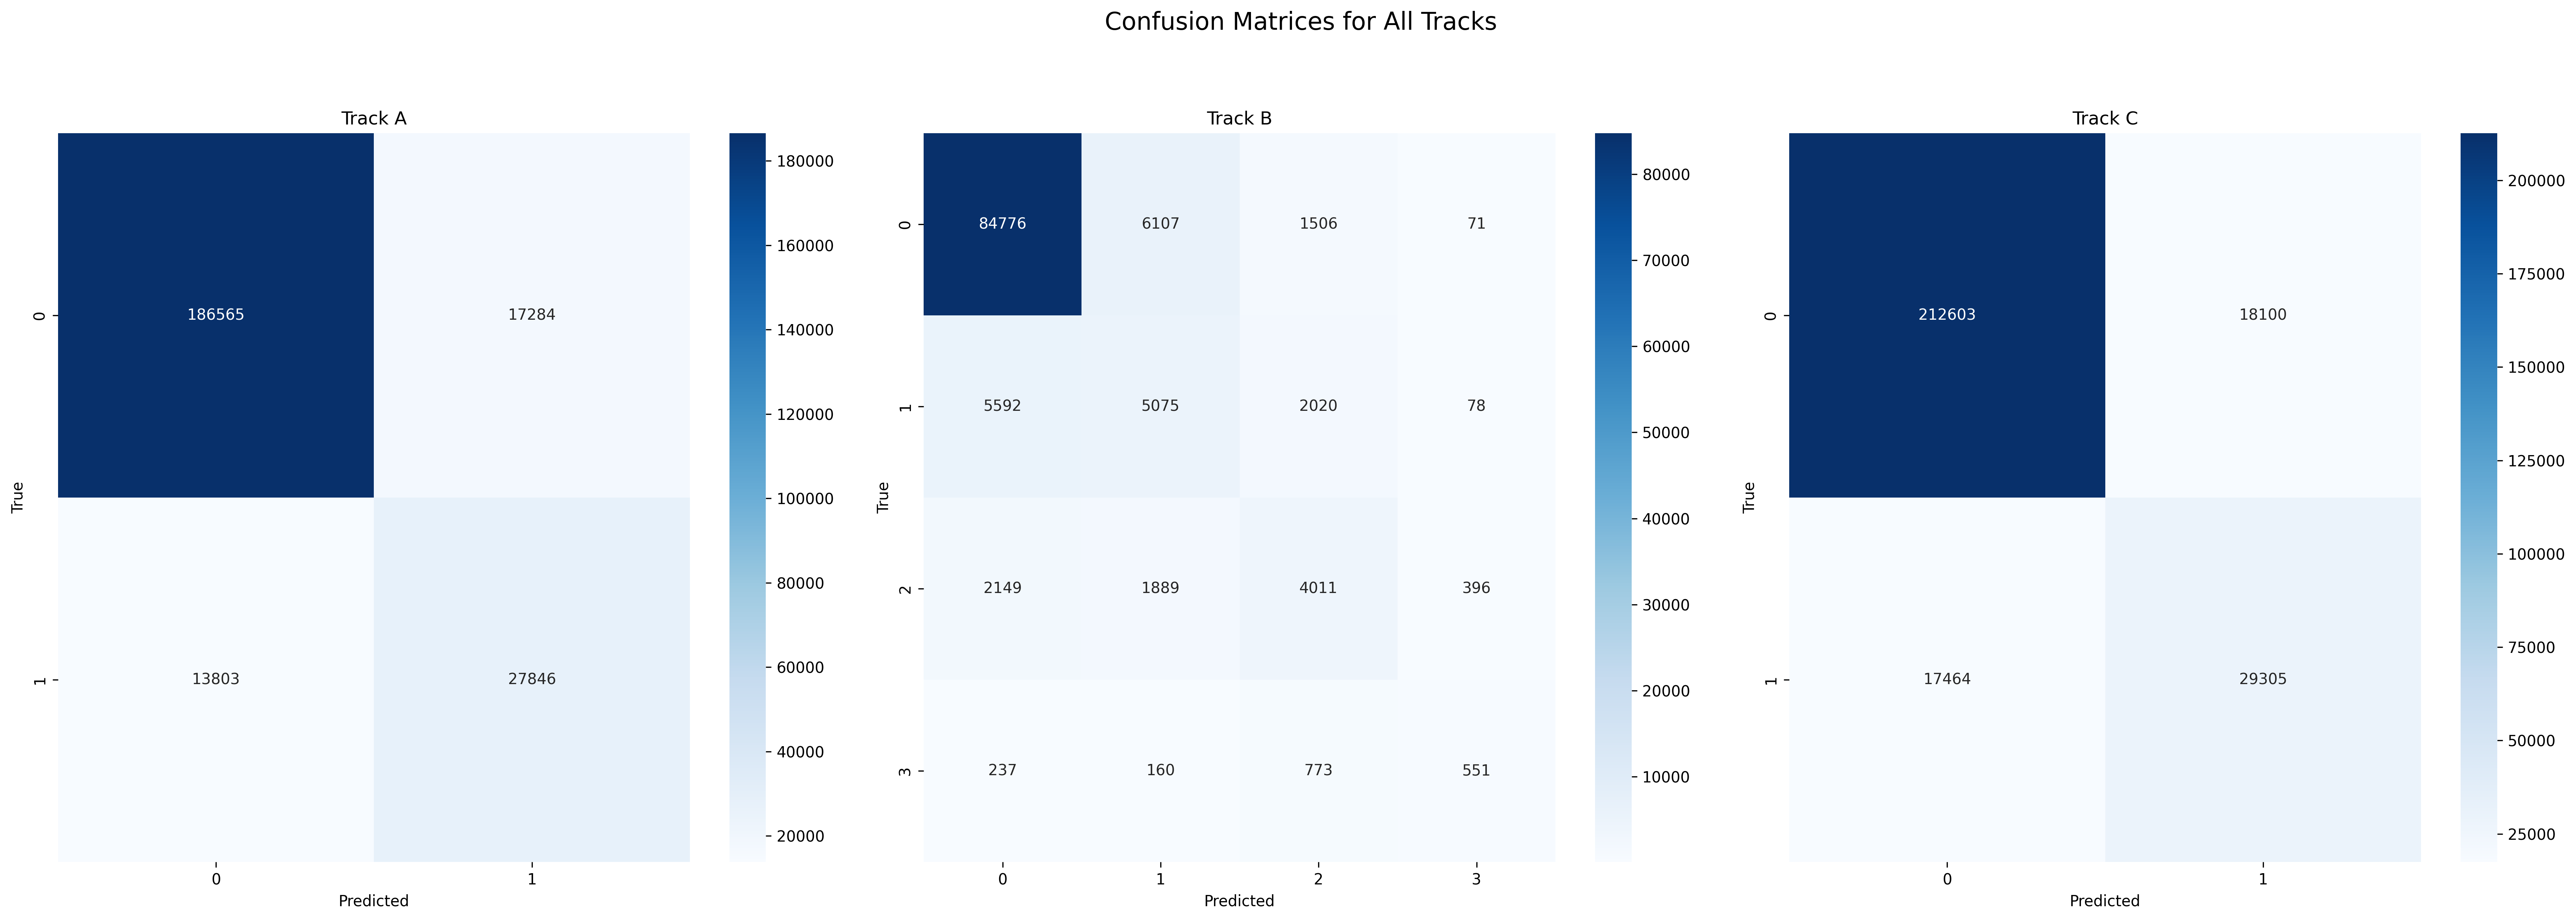
\includegraphics[width=1.7\columnwidth]{images/confusion_matrices_all_tracks.png}
    \caption{Confusion matrices for each language across Tracks A, B, and C.}
    \label{fig:confusion_matrices}
\end{figure*}

\subsection{Data Splits and Usage}
The dataset\cite{muhammad2025brighterbridginggaphumanannotated} was divided into three subsets: training, development (validation), and testing. Specifically, 80\% of the training dataset was allocated for training, while the remaining 20\% was reserved for validation to facilitate model selection. Once the best-performing model was identified during the validation phase, the entire training and development datasets were combined to retrain the final model. This final model was then evaluated on the test dataset, which was held out during the entire training process to ensure an unbiased assessment of the model's generalization performance. This approach adheres to standard practices in machine learning research to prevent data leakage and ensure robust evaluation \citep{Goodfellow-et-al-2016}.

\subsection{Preprocessing}

Preprocessing of the dataset was performed using the \texttt{clean-text} library. The preprocessing pipeline involved multiple steps to clean and standardize the text data. Initially, all text was converted to lowercase, and unnecessary whitespace was removed to eliminate redundancy. Special characters, URLs, and emojis were filtered out using regular expressions. Emojis were replaced by their corresponding textual descriptions (e.g., \smiley $\rightarrow$ ``smiling face''). Punctuation was also removed, and  tokenization was performed using language-specific tokenizers to ensure optimal segmentation, and stopwords were removed to further reduce noise. These steps ensured the data was clean and consistent across all subsets. Preprocessing was applied consistently to the training, validation, and test datasets to avoid introducing biases or inconsistencies. Such preprocessing steps have been shown to improve the performance of NLP models by reducing noise and simplifying the input representations \citep{Zhang2020DataPrep}.

\subsection{Hyperparameter Tuning}

Hyperparameter tuning used Optuna \citep{Akiba2019Optuna} to optimize SVM and XGBoost hyperparameters. Bayesian optimization balanced exploration and exploitation, with configurations assessed on the validation set. The best configuration was selected based on the performance metric.

\subsection{Model Training and Optimization}

The model fine-tuning with LoRA, and the training of the MLP and XGBoost models, utilized Binary Cross-Entropy (BCE) as the loss function for Tracks A and C, and Cross-Entropy for Track B, owing to its appropriateness for classification tasks. Meanwhile, the training of the SVM model employed hinge loss.Using LoRA, we fine-tuned the Q, K, and V matrices for feature extractor transformer models, as shown in Table \ref{tab:model_selection}. Given the unbalanced dataset, a weighted loss approach was employed to ensure that the model adequately learned from all classes. Optimization for fine-tuning deep learning models was performed using the \texttt{AdamW} optimizer, which improves upon the standard Adam optimizer by decoupling weight decay and learning rate updates \citep{Loshchilov2019AdamW}. To further enhance training stability and convergence, a cosine annealing learning rate scheduler with restarts\cite{loshchilov2017sgdrstochasticgradientdescent} was employed. This scheduling approach helped adaptively reduce the learning rate over time, facilitating better exploration of the loss landscape and improving generalization. The model was trained for a fixed number of epochs, and early stopping was used to terminate training if the validation performance plateaued, thus avoiding overfitting.
\begin{table*}[h!]
    \centering
    \resizebox{2\columnwidth}{!}{
        \begin{tabular}{|p{12cm}|c|c|c|c|c|c|}
            \hline
            \textbf{Text}                                                                                                                                                                                                                                                                           & \textbf{Type} & \textbf{Anger} & \textbf{Fear} & \textbf{Joy} & \textbf{Sadness} & \textbf{Surprise} \\ \hline
            \multirow{2}{12cm}{I'm just numb.}                                                                                                                                                                                                                                                      & Truth         & 0              & 0             & 0            & 1                & 0                 \\ \cline{2-7}
                                                                                                                                                                                                                                                                                                    & Pred          & 0              & 1             & 0            & 1                & 0                 \\ \hline
            \multirow{2}{12cm}{At the time it didn't seem to bother me.}                                                                                                                                                                                                                            & Truth         & 0              & 0             & 0            & 1                & 0                 \\ \cline{2-7}
                                                                                                                                                                                                                                                                                                    & Pred          & 0              & 0             & 0            & 0                & 0                 \\ \hline
            \multirow{2}{12cm}{I found out six weeks before                                                                                                                     the wedding that my dad had only six weeks to live (he had cancer for two years... a fact she was fully aware of).} & Truth         & 1              & 1             & 0            & 1                & 1                 \\ \cline{2-7}
                                                                                                                                                                                                                                                                                                    & Pred          & 0              & 1             & 0            & 1                & 0                 \\ \hline
        \end{tabular}
    }
    \caption{Error Analysis Table of language English for track A}
    \label{tab:error_analysis}
\end{table*}


\subsection{Tools and Libraries}

The implementation of the experiments utilized several state-of-the-art tools and libraries. The deep learning models were implemented and trained using \texttt{PyTorch} \citep{Paszke2019PyTorch}. For data manipulation and evaluation metrics, \texttt{Scikit-Learn} was employed \citep{Pedregosa2011ScikitLearn}. Gradient boosting models were benchmarked using \texttt{XGBoost} \citep{chen2016xgboost}. Pre-trained transformer models were fine-tuned using \texttt{Hugging Face Transformers} \citep{Wolf2019HuggingFace}. Additionally, the \texttt{Sentence Transformers} library was used to load embedding models \cite{reimers-2019-sentence-bert}\cite{reimers-2020-multilingual-sentence-bert}. These tools and libraries are well-regarded in the machine learning community and were chosen for their reliability and performance.

\subsection{Computational Resources}

Experiments used a Kaggle Tesla P100 GPU for efficient model training, evaluation, and hyperparameter tuning, ensuring reproducibility with comparable hardware.

% \subsection{Postprocessing}

% Postprocessing involved thresholding the model's output probabilities to convert them into binary class predictions. A default threshold of 0.5 was used, but sensitivity analyses were conducted to evaluate the impact of varying the threshold. This ensured that the model's performance was robust across different operating points and provided interpretable results for downstream tasks. Minimal additional postprocessing was applied to maintain the integrity of the model's predictions.

% \subsection{Concluding Remarks on Setup}

% The experimental setup was designed to maximize the reliability, reproducibility, and validity of the results. By adhering to established best practices in data splitting, preprocessing, and hyperparameter tuning, and by leveraging state-of-the-art tools and optimization strategies, the experimental methodology ensures a robust evaluation of the model's performance. Furthermore, the combination of advanced optimization techniques, careful preprocessing, and systematic model selection contributes to the study's alignment with the broader goals of advancing research in machine learning. This setup not only facilitates a fair comparison with existing methods but also provides a strong foundation for further exploration and improvement of the proposed approach.